\documentclass{article}
\usepackage[utf8]{inputenc}
\usepackage[usenames,svgnames]{xcolor}

% Page setup
\usepackage[a4paper,landscape,margin=2cm]{geometry}
\usepackage{amsmath}

% Typography
\usepackage[scaled]{helvet}
\let\familydefault\sfdefault


\usepackage{tikz,pgfplots,tikzpeople,tikz-layers}
\usetikzlibrary{positioning,arrows,intersections,calc,fit,shapes}

\definecolor{colorwhite}    {RGB}{255,255,255}
\definecolor{colorpod}      {RGB}{199,212,104}
\definecolor{colorbook}     {RGB}{ 79,142,209} 
\definecolor{colorprofile}  {RGB}{143,232,186}
\definecolor{colortext}     {RGB}{ 29, 29, 27}
\definecolor{colorkey}      {RGB}{129, 29, 27}
\definecolor{colorperson}   {RGB}{190, 22, 34}

\makeatletter
\pgfdeclareshape{datastore}{
  \inheritsavedanchors[from=rectangle]
  \inheritanchorborder[from=rectangle]
  \inheritanchor[from=rectangle]{center}
  \inheritanchor[from=rectangle]{base}
  \inheritanchor[from=rectangle]{north}
  \inheritanchor[from=rectangle]{north east}
  \inheritanchor[from=rectangle]{east}
  \inheritanchor[from=rectangle]{south east}
  \inheritanchor[from=rectangle]{south}
  \inheritanchor[from=rectangle]{south west}
  \inheritanchor[from=rectangle]{west}
  \inheritanchor[from=rectangle]{north west}
  \backgroundpath{
    %  store lower right in xa/ya and upper right in xb/yb
    \southwest \pgf@xa=\pgf@x \pgf@ya=\pgf@y
    \northeast \pgf@xb=\pgf@x \pgf@yb=\pgf@y
    \pgfpathmoveto{\pgfpoint{\pgf@xa}{\pgf@ya}}
    \pgfpathlineto{\pgfpoint{\pgf@xb}{\pgf@ya}}
    \pgfpathmoveto{\pgfpoint{\pgf@xa}{\pgf@yb}}
    \pgfpathlineto{\pgfpoint{\pgf@xb}{\pgf@yb}}
 }
}
\makeatother

\begin{document}
\pagestyle{empty}

% ======================================= V


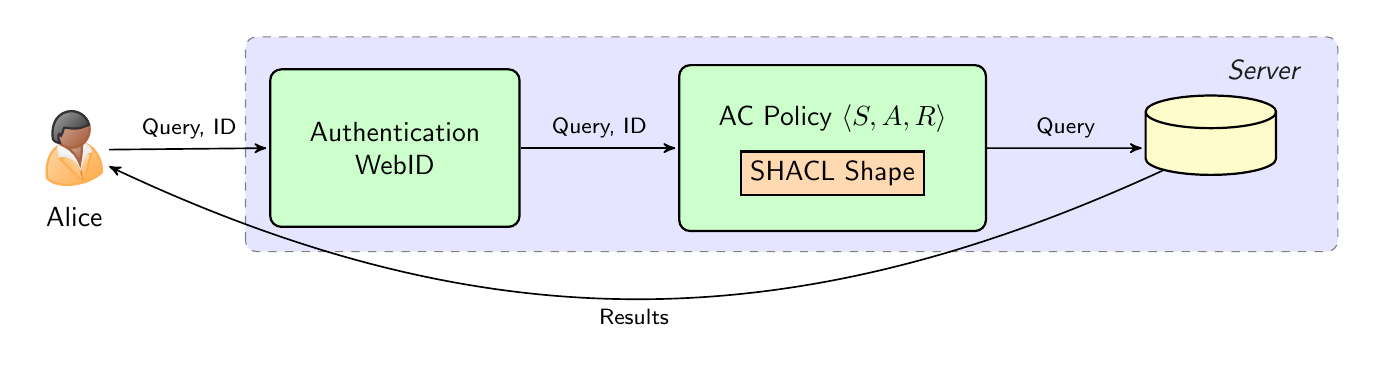
\begin{tikzpicture}[
    node distance = 10em, auto, thick,
    title/.style={text=colortext,font={\Large\itshape}},
    person/.style={text=colorwhite,font={\Large\bfseries}},
    code/.style={text=colortext,font={}},
    key/.style={text=colorkey,font={\tiny\itshape}},
    every matrix/.style={ampersand replacement=\&,column sep=2cm,row sep=2cm},
    source/.style={draw,thick,rounded corners,fill=yellow!20,inner sep=.3cm},
    db/.style={draw,thick,fill=yellow!20},
    process/.style={draw,thick,circle,fill=blue!20},
    sink/.style={source,fill=green!20,inner sep=.5cm, minimum height=2cm},
    datastore/.style={draw,very thick,shape=datastore,inner sep=.3cm},
    dots/.style={gray,scale=2},
    to/.style={->,>=stealth',shorten >=1pt,semithick,font=\sffamily\footnotesize},
    every node/.style={align=center}]
  
    % % Position the nodes using a matrix layout
    % \& \node[datastore] (buffer) {buffer};  \& \\
  
    % \node[datastore] (storage) {storage};     \& \node[process] (monitor) {monitor};  \& \node[sink] (datastore) {datastore}; \\
    \matrix{
      \node[alice,minimum size=2em,label={[label distance=0.1em]below:Alice}] (ALICE){}; \& \node[sink] (AW) {Authentication \\ WebID}; \& \node[sink] (ACP) {AC Policy $\langle S,A,R\rangle$\\\\}; \& \node[db,cylinder,shape border rotate=90,shape aspect=.25, text opacity=0] (DS) {\phantom{Datastore}};\\
    };
    \node[draw,fill=orange!30] at ([yshift=0.75cm]ACP.south){SHACL Shape};
    % Draw the arrows between the nodes and label them.
    \draw[to] (ALICE) -- node[midway,above] {Query, ID} (AW);
    \draw[to] (AW) -- node[midway,above] {Query, ID} (ACP);
    \draw[to] (ACP) -- node[midway,above] {Query} (DS);
    \draw[to] (DS) to[bend left=25] node[midway,below] {Results} (ALICE);

    \begin{scope}[on behind layer]
            \path (AW.south west)+(-0.3,-0.3) node (a2) {};
        \path (DS.north east)+(1,0.8) node (b2) {};
		\draw[fill=blue!10,rounded corners, draw=black!50, dashed]
      (a2) rectangle (b2);
      \node[title,font={\itshape},above right=0.4em and -1.5em of DS] {Server};

      \end{scope}
\end{tikzpicture}
\end{document}
